%%%%% Paramétrage du cours %%%%
%\def\xxactivite{Cours}
%\def\xxauteur{\textsl{Xavier Pessoles}}
%
%\fichetrue
%\proftrue
%\tdfalse
\setchapterimage{Header_Peugeot.jpg}
\setchapterpreamble[u]{\margintoc}
%\setcounter{chapter}{1}

\chapter{Résolution d'un problème de dynamique}

\marginnote[3cm]{
\UPSTIcompetence[2]{C1-05}
\UPSTIcompetence[2]{C2-08}
\UPSTIcompetence[2]{C2-09}
%\UPSTIcompetence[2]{C2-03}
}


\setcounter{section}{0}
\section{Ce qu'il faut connaître et savoir faire... pour pouvoir commencer}
\begin{enumerate}
\item \textbf{Faire un graphe d'analyse (ou de structure : liaisons et actions mécaniques extérieures).}
\item \textbf{Faire un bilan des actions mécaniques extérieures et écrire le torseur associé.}
\item \textbf{Les torseurs des actions mécaniques dans les liaisons.}
\item \textbf{Simplifier les torseurs des actions mécaniques dans les liaisons dans le cas d'un problème plan}.
\item \textbf{Faire des produits vectoriels le plus vite possible.}
\item \textbf{Calculer un torseur dynamique}.
\end{enumerate}



\section{Les types de problèmes}

Le principe fondamental de la dynamique a pour objectif de :
\begin{enumerate}
\item \textbf{déterminer une loi de mouvement;}
\item \textbf{déterminer les actions mécaniques dans les liaisons}.
\end{enumerate}

Le cas 1 est le plus souvent rencontré. L'objectif est de trouver une équation différentielle \textbf{indépendamment des actions dans les liaisons} et liant positions, vitesses, accélérations, dimensions et propriétés massiques. 
Cette loi permet généralement de dimensionner les actionneurs d'un système (couple moteur ou effort à fournir par un actionneur linéaire -- vérin par exemple --).

Dans le cas 2, on peut essayer de minimiser le nombre d'équations à écrire. C'est cette stratégie que nous allons présenté.

Dans le cas 2, il faut isoler chacune des pièces et réaliser le PFD. 




\section{Stratégie d'isolement}

\subsection{Graphe d'analyse, ou de structure}

On rencontre principalement deux types de structures : des chaînes fermées, ou des chaînes ouvertes.

\begin{figure*}[!ht]
\begin{minipage}[c]{.4\linewidth}
\begin{center}
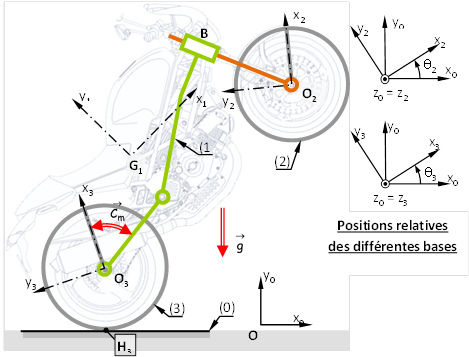
\includegraphics[width=\linewidth]{fig_01}
\end{center}
\end{minipage}
\hfill
\begin{minipage}[c]{.55\linewidth}
\begin{center}
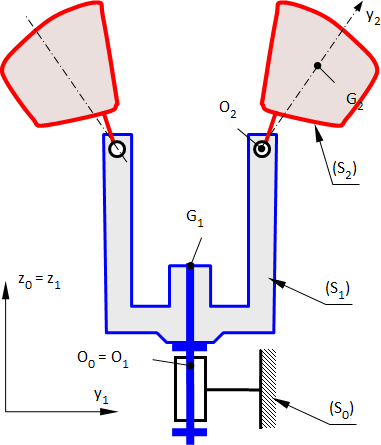
\includegraphics[width=\linewidth]{fig_02}
\end{center}
\end{minipage}
\end{figure*}

\textbf{Remarques :}
\begin{itemize}
\item Entre les pièces (ou les groupes de pièces), on matérialise les liaisons (dont vous connaissez super bien les torseurs).
\item Entre certaines pièces (ou groupes de pièces), il peut exister des actions mécaniques extérieures qui agissent << en positif >> sur une des pièces et << en négatif~>> sur l'autre. \textbf{C'est par exemple le cas des moteurs et des vérins}. Il faut bien préciser que l'action mécanique agit sur les deux pièces.
\item Les actions strictement extérieures (comme la pesanteur) ne sont pas en interactions entre deux pièces.
\end{itemize}


\subsection{Isoler les solides soumis à 2 glisseurs}

On commence toujours, \large{toujours}, \Large{toujours}, \LARGE{toujours}, \huge{toujours} \normalsize par isoler les ensembles soumis à 2 glisseurs... Mais cela vous le saviez :). Cependant, en dynamique ce cas est rare. On peut le rencontrer, dans le cas des problèmes plans, lorsque la masse d'un solide est négligée.


\subsection{Cas des chaînes ouvertes}

\begin{marginfigure}
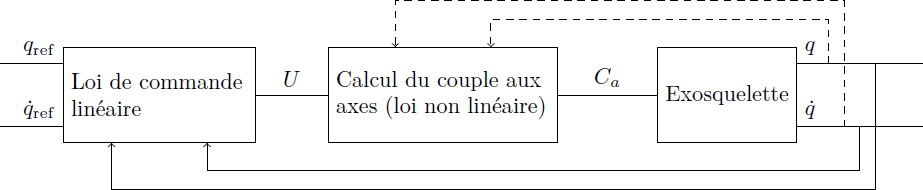
\includegraphics[width=\linewidth]{fig_06}
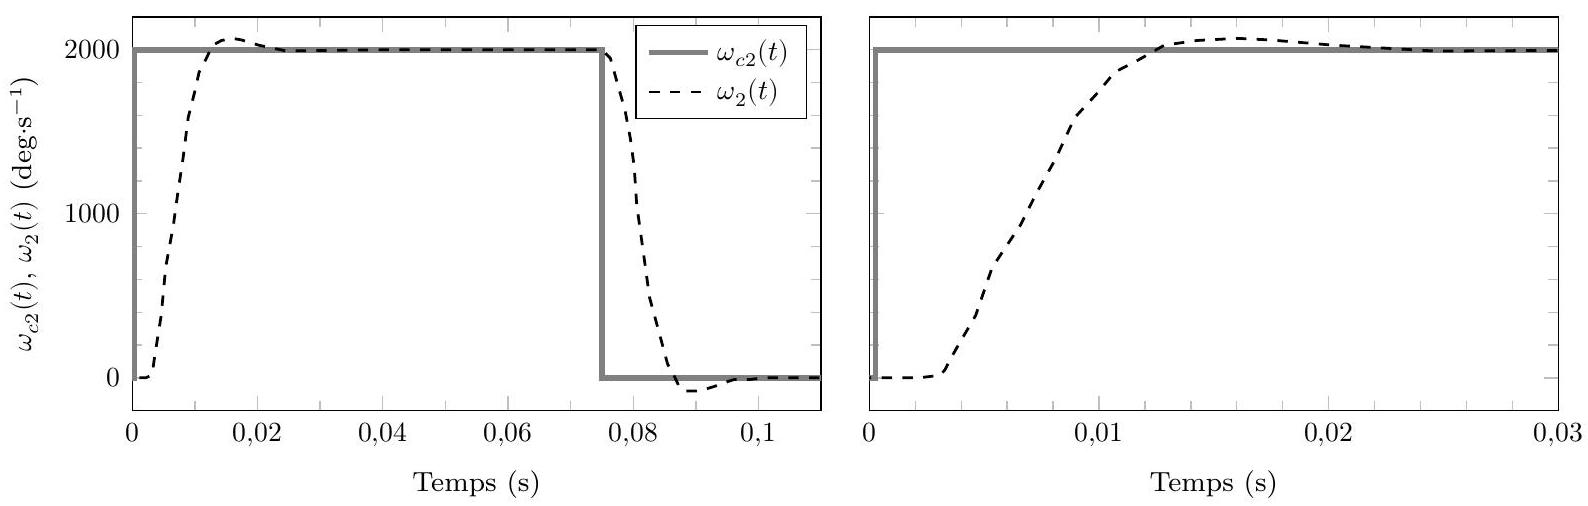
\includegraphics[width=\linewidth]{fig_07}
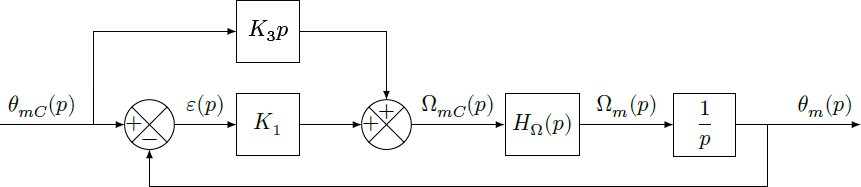
\includegraphics[width=\linewidth]{fig_08}
\end{marginfigure}

C'est le cas le plus rencontré en dynamique. 

On commence par isoler le bout de chaîne. Puis on réalise le théorème correspondant à a mobilité de cet ensemble et on poursuit le raisonnement. 



Ainsi, pour la figure ci-contre :
\begin{enumerate}
\item pour obtenir $C_{m3}$, on isole 4 et on fait un théroème du moment dynamique en $C$ en projection sur $\vz{}$;
\item pour obtenir $C_{m2}$, on isole \{4+3\} et on fait un théroème du moment dynamique en $B$ en projection sur $\vy{}$;
\item pour obtenir $F_{v}$, on isole \{4+3+2\} et on fait un théroème de la résultante dynamique en projection sur $\vx{}$.
\end{enumerate}


\subsection{Cas des chaînes fermées}

Ce cas n'est pas le plus fréquent. Lorsqu'on désire obtenir la loi de mouvement d'une chaîne fermée, il est généralement plus rapide d'uiliser le théorème de l'énergie cinétique que nous aborderons plus tard. 

Pous les chaînes fermées, on va réaliser une coupure << fictive >> dans le système et reprendre la méthode précédente. 

L'objectif et que toutes les équations dynamiques fassent apparaître les inconunes statiques d'une seule et même liaisons. Cela permettra finalement de disposer d'assez d'équations pour supprimer ces inconnues de liaisons.

\begin{marginfigure}
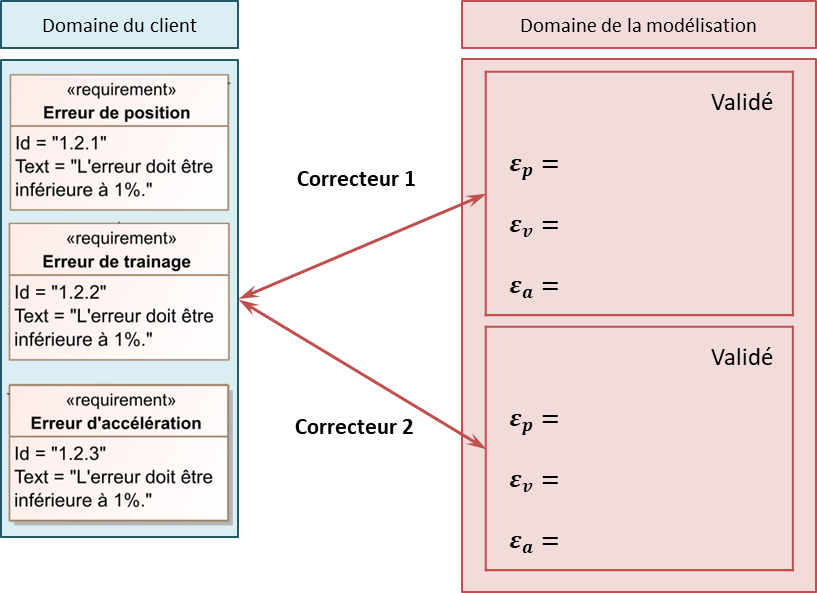
\includegraphics[width=\linewidth]{fig_09}
\end{marginfigure}

Pour l'exemple ci-contre : 
\begin{enumerate}
\item on isole 4 et on réalise un théorème de la résultante dynamique en projection sur $\vy{}$;
\item on isole 3 et on réalise un théorème du moment dynamique en $B$ en projection sur $\vz{}$;
\item on isole \{2+3\} et on réalise un théorème du moment dynamique en $A$ en projection sur $\vz{}$.
\end{enumerate}



\subsection{Cas des véhicules}
Dans les cas des véhicules, l'application du PFD permet de déterminer 
\begin{itemize}
\item les conditions de dérapages en ligne droite ou en virage;
\item les conditions de basculent en ligne droite ou en virage.
\end{itemize}

\subsubsection{Véhicule qui accélère, sans glissement des roues}

\begin{marginfigure}
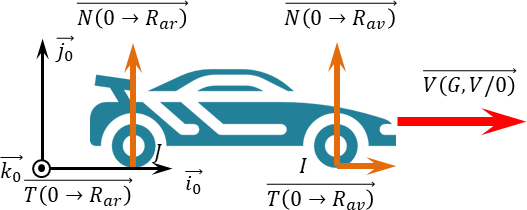
\includegraphics[width=\linewidth]{fig_10}
\caption{Véhicule en mouvement \label{fig:fig_10}}
\end{marginfigure}

La figure \ref{fig:fig_10} permet de modéliser (partiellement) les actions mécaniques sur un véhicule en ligne droite.  En faisant les hypothèses suivantes : 
\begin{itemize}
\item véhicule qui accélère et roues avant motrices, 
\item problème plan;
\item masse des roues négligeables;
\end{itemize}
il en résulte que la roue arrière (dont l'inertie est nulle si la masse est négligeable) est soumise à deux glisseurs (pivot dans le plan avec le châssis et contact ponctuel avec le sol). En conséquence, il n'y a pas d'effort tangentiel dans cette liaison. 

De plus en phase d'accélération et d'adhérence de la roue avant, l'effort tangentiel de la roue sur le sol est vers l'avant. 

\subsubsection{Freinage, roues bloquées}

\begin{marginfigure}
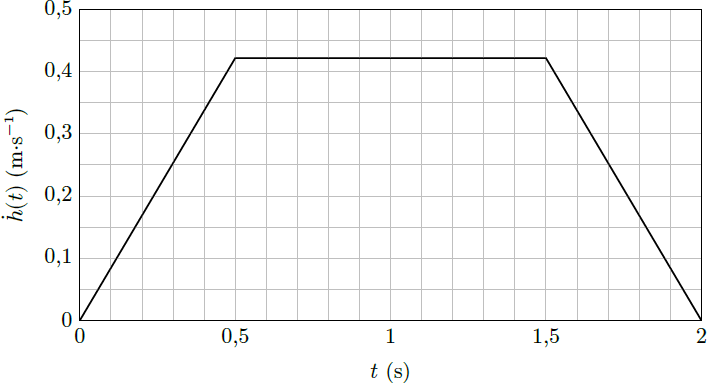
\includegraphics[width=\linewidth]{fig_11}
\caption{Freinage et glissade ... \label{fig:fig_11}}
\end{marginfigure} 

On se met dans le cas d'un freinage sur toutes les roues et ces roues se bloquent. Le véhicule glisse et l'effort tangentiel s'oppose au mouvement. On est dans le cas d'un glissement, donc on est sur le cône de frottement. 

La loi de mouvement peut s'obtenir en isolant tout le véhicule et en réalisant un \textbf{théorème de la résultante dynamique} suivant $\vi{0}$. Le TRD sur $\vj{0}$, le TMD (par exemple en $I$) et les lois de Coulomb permettent de supprimer les inconnues de liaison.


\begin{marginfigure}
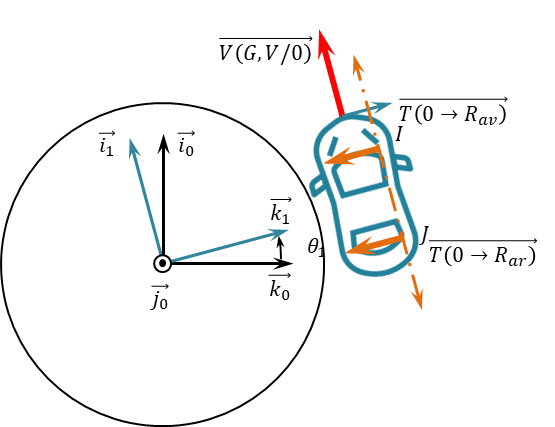
\includegraphics[width=\linewidth]{fig_13}
\caption{Dérapage \label{fig:fig_13}}
\end{marginfigure} 

\subsubsection{Dérapage en rond point}

Si on dérape (figure \ref{fig:fig_13)}), c'est nécessairement suivant la direction $\vk{1}$. La loi de mouvement, ou les conditions de dérapge, peuvent s'obtenir en isolant tout le véhicule et en réalisant un \textbf{théorème de la résultante dynamique} suivant $\vi{0}$. 
La tendance au dérapement étant vers l'extérieur du virage, les efforts tangentiels sont nécessairement orientés vers l'intérieur du virage.


\subsubsection{Tonneau en rond point}

\begin{marginfigure}
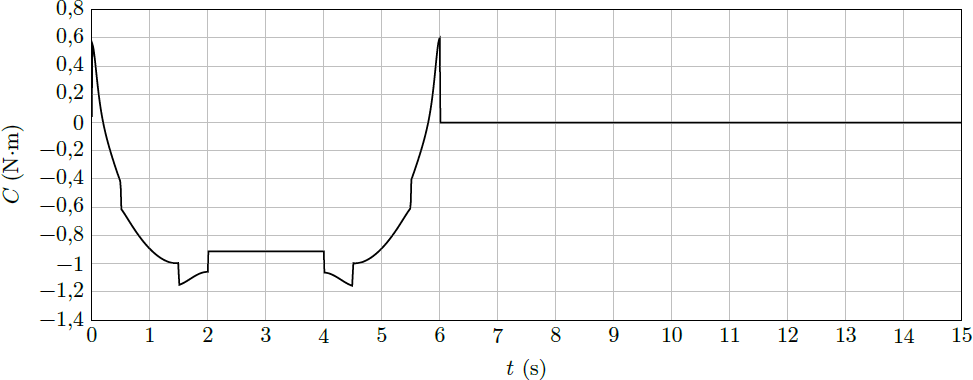
\includegraphics[width=\linewidth]{fig_12}
\caption{Tonneau \label{fig:fig_12}}
\end{marginfigure} 


Si la voiture part en tonneau (figure \ref{fig:fig_12)} c'est nécessairement en pivotant autour de l'axe $\vect{IJ}$. Pour déterminer les conditions de tonneau, il faudra donc d'une part réaliser un \textbf{théorème du moment dynamique} en $I$ ou en $J$ en projection suivant la direction $\vect{IJ}$ (c'est-à-dire vecteur $\vi{1}$). 
\textbf{On cherchera alors la condition où les efforts normaux sur les roues intérieures seront nulles.}



\subsubsection{Wheeling en moto}

\begin{marginfigure}
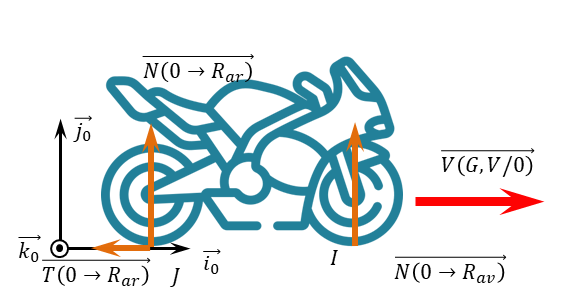
\includegraphics[width=\linewidth]{fig_15}
\caption{Wheeling \label{fig:fig_15}}
\end{marginfigure} 

On souhaite savoir dans quelles conditions il est possible de faire un wheeling en moto, c'est à dire pour quelle accélération, la roue avant va se décoller du sol. 
Ce mouvement correspond à une rotation de la moto autour de la roue arrière.

Pour traduire ce mouvement, on isole l'ensemble de la moto et on réalise un \textbf{théorème du moment dynamique} en $J$ en on détermine \textbf{à quelle condition l'effort normal sur la roue avant est nul}.



\subsubsection{Soleil en moto}

\begin{marginfigure}
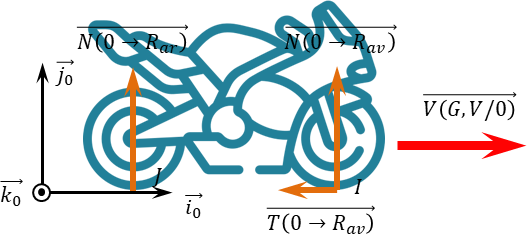
\includegraphics[width=\linewidth]{fig_16}
\caption{Soleil \label{fig:fig_16}}
\end{marginfigure} 

On souhaite savoir dans quelles conditions il est possible de décoler la roue arrière, c'est à dire pour quelle délération, la roue arrière va se décoller du sol lors d'un freinage sur la roue avant uniquement (roue avant bloquée).
Ce mouvement correspond à une rotation de la moto autour de la roue avant.

Pour traduire ce mouvement, on isole l'ensemble de la moto et on réalise un \textbf{théorème du moment dynamique} en $I$ en on détermine \textbf{à quelle condition l'effort normal sur la roue arrière est nul}.

\subsection{Il y a plus qu'à ...}
\subsubsection{Produit mixte}
Petite remarque pour finir : le produit mixte. Lorsqu'on applique un théorème suivant une direction, le produit mixte peut être un bon outil :
$\vectm{B}{1}{2}\cdot \vect{z} = \left( \vectm{A}{1}{2} + \vect{BA}\wedge \vectf{1}{2}\right)\cdot \vect{z}$
$=  \vectm{A}{1}{2}\cdot \vect{z} + \left(\vect{BA}\wedge \vectf{1}{2}\right)\cdot \vect{z}$...
et $\left(\vect{u} \wedge \vect{v}\right) \cdot \vect{z}= \left(\vect{v} \wedge \vect{z}\right) \cdot \vect{u}= \left(\vect{z} \wedge \vect{u}\right) \cdot \vect{v}$.

\subsubsection{Projection de la dérivée et dérivée de la projection...}
\marginnote{On reconnaîtra que $(uv)' = u'v + uv'$ et donc $u'v =  (uv)' -u v' $.}
On pourra utiliser judicieusement le résultat suivant : 
$$
\deriv{\vect{V}(t)}{\bas{0}}\cdot \vect{u}(t) =
\deriv{\vect{V}(t) \cdot \vect{u}(t) }{} - \vect{V}(t) \cdot \deriv{\vect{u}(t)}{\bas{0}} 
$$

\section{Loi de mouvement}

En règle générale, les lois de mouvement permettent d'exprimer le couple moteur ou l'effort à fournir pour un vérin pour réaliser un déplacement. Ces lois sont des équations différentielles d'ordre 2. En général, il n'est pas nécessaire de résoudre ces équations différentielles car le mouvement est forcé par la commande. 

Une des lois usuellement suivie par un actionneur pour aller d'un point à un autre est une loi de mouvement de vitesse en trapèze.  Ce mouvement peut être décomposé en 3 phases : 
\begin{itemize}
\item phase 1 mouvement uniformément décéléré. L'accélération est donc constante, la vitesse croit de façon linéaire et la position de façon parabolique;
\item phase 2 : mouvement uniforme. L'accélération est nulle, la vitesse est constante et la position évolue linéairement;
\item phase 3 : mouvement uniformément décéléré. L'accélération est constante est négative, la vitesse décroît linéairement et la position évolue de façon parabolique. 
\end{itemize}

\begin{marginfigure}
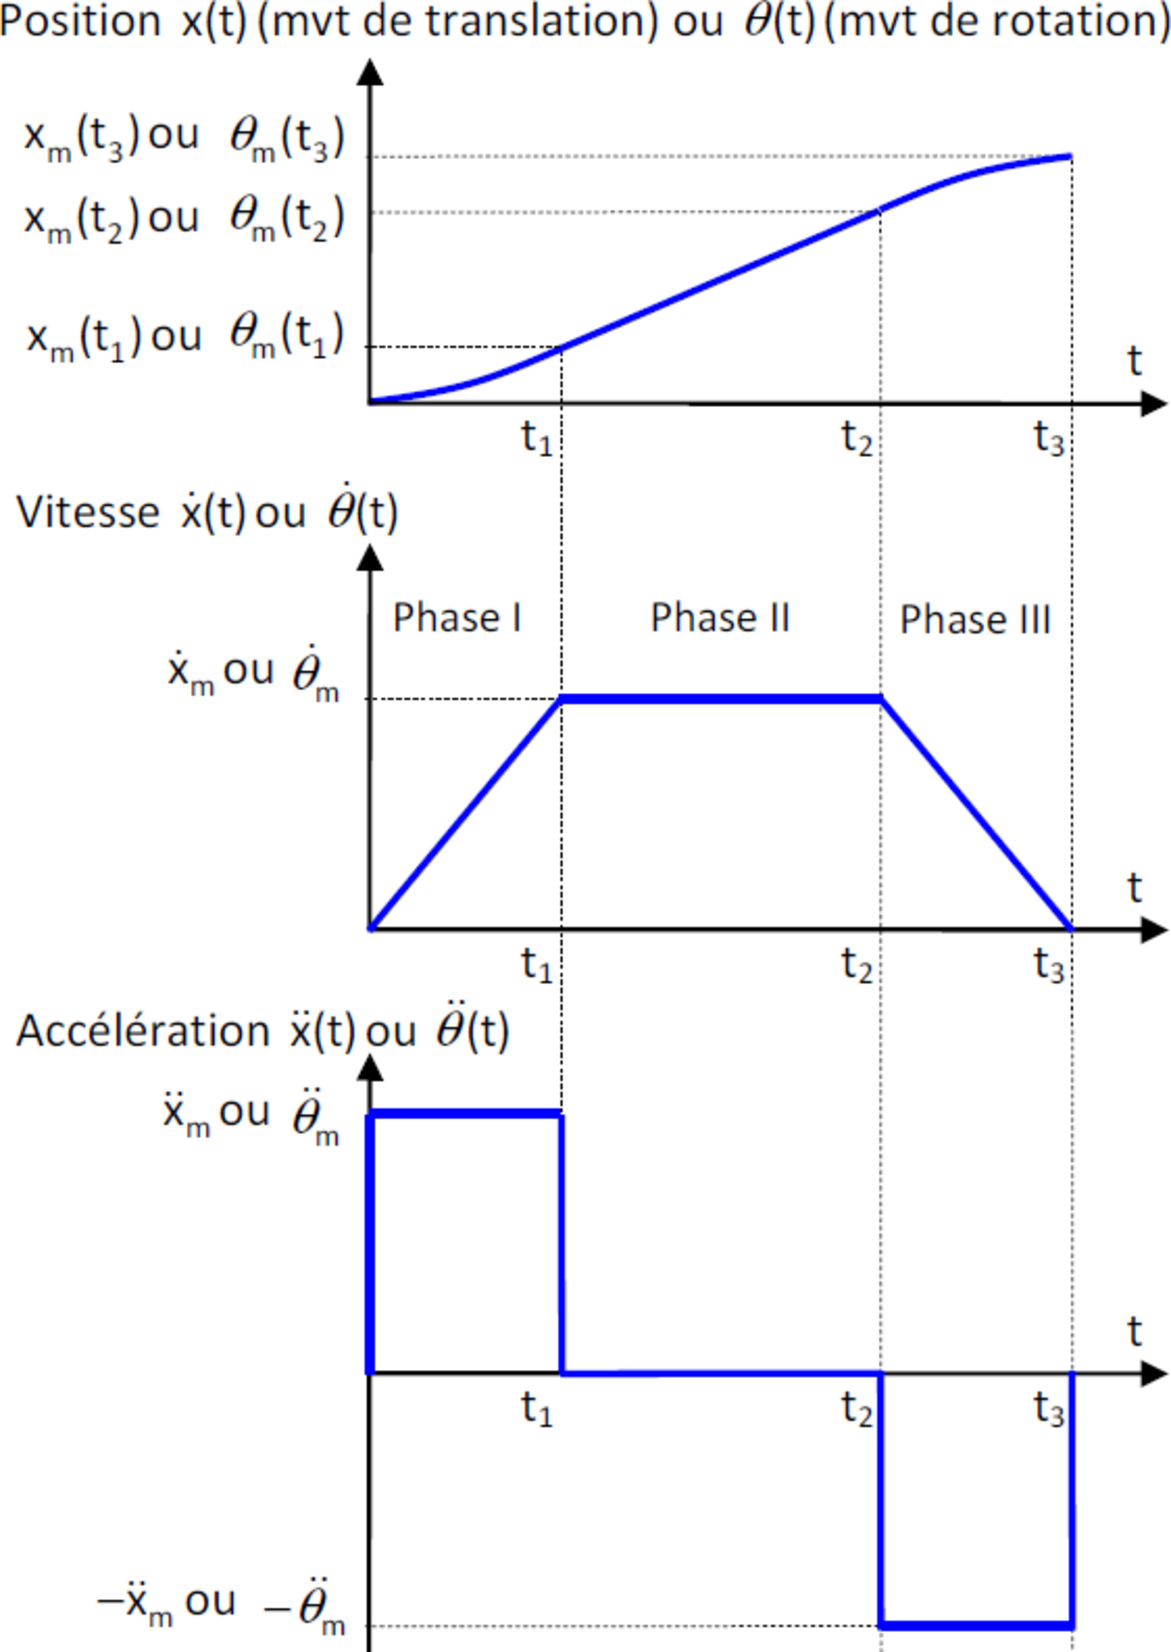
\includegraphics[width=\linewidth]{trapeze}
\end{marginfigure}


Dans le cas général, il sera souvent inutile d'écrire les équations horaires de chacune des phases. En effet, les questions liées à ces lois de mouvements sont généralement :
\begin{itemize}
\item d'identifier le << pire des cas >> en terme de vitesse/accélération;
\item de déterminer les temps de une ou plusieurs des phases en fonction de la distance à parcourir, la vitesse maximale, l'accélération accélérations maximale;
\item de déterminer la hauteur du palier de vitesse;
\item de déterminer la distance parcourue. 
\end{itemize}


\begin{resultat}
Dans les 3 derniers points, il est souvent suffisant de remarquer en utilisant les courbes que : 
\begin{itemize}
\item $t_1=\dfrac{\dot{x}_m}{\ddot{x}_m}$;
\item en utilisant la courbe de vitesse et en remarquant que l'intégrale sous la courbe correspond à la distance parcourue, la distance parcourue lors de l'accélération est donnée par $\dfrac{1}{2}t_1\dot{x}_m$;
\item en utilisant la courbe de vitesse et en remarquant que l'intégrale sous la courbe correspond à la distance parcourue, la distance parcourue lors des 3 phases est donnée par $2\cdot \dfrac{1}{2}t_1\dot{x}_m+\left(t_2-t_1\right)\dot{x}_m$.
\end{itemize}
\end{resultat}


\begin{center}
\begin{tabular}{|p{2.2cm}|c|c|c|}
\hline
 & Phase 1 & Phase 2 & Phase 3 \\
\hline \hline
Équation de position & 
$x(t)=\dfrac{1}{2}\ddot{x}_mt^2 $ &
$x(t)= \dot{x}_m(t)\left( t-t_1\right)+x_m\left(t_1 \right)$ & 
$x(t)= -\dfrac{1}{2}\ddot{x}_m\left(t-t_2\right)^2 + \dot{x}_m(t)\left( t-t_2\right)+x_m\left(t_2\right)$ \\ \hline
Équation de vitesse &
$\dot{x}(t)=\ddot{x}_m t$ &  
$\dot{x}(t)=\dot{x}_m $ & 
$\dot{x}(t)=-\ddot{x}_m \left(t-t_2\right)+\dot{x}_m$  \\ \hline
Équation d'accélération &
$\ddot{x}(t)=\ddot{x}_m$ & 
$\ddot{x}(t)=0$ & 
$\ddot{x}(t)=-\ddot{x}_m$ \\
\hline
\end{tabular}
\end{center}
